%%%%%%%%%%%%%%%%%%%%%%%%%%%%%%%%%%%%%%%%%%%%%%%%%%%%%%%
%% Bachelor's & Master's Thesis Template             %%
%% Copyleft by Artur M. Brodzki & Piotr Woźniak      %%
%% Covered for Lab/Assigment report by Tymon Żarski  %%
%% Faculty of Electronics and Information Technology %%
%% Warsaw University of Technology, 2019-2020        %%
%%%%%%%%%%%%%%%%%%%%%%%%%%%%%%%%%%%%%%%%%%%%%%%%%%%%%%%

\documentclass[
    left=2.5cm,         % Sadly, generic margin parameter
    right=2.5cm,        % doesnt't work, as it is
    top=2.5cm,          % superseded by more specific
    bottom=3cm,         % left...bottom parameters.
    bindingoffset=6mm,  % Optional binding offset.
    nohyphenation=false % You may turn off hyphenation, if don't like.
]{eiti/eiti-report}

\usepackage{listings}

\langpol % Dla języka angielskiego mamy \langeng
\graphicspath{{img/}}             % Katalog z obrazkami.
\addbibresource{bibliografia.bib} % Plik .bib z bibliografią

\begin{document}

%--------------------------------------
% Strona tytułowa
%--------------------------------------
\instytut{XXXXXX}
\przedmiot{Wprowadzenie do przetwarzania języka naturalnego}
\specjalnosc{XXXXXX}
\title{
    Analiza wydźwięku w języku angielskim na bazie recenzji produktów
}
\reportDescription{
    Dokumentacja wstępna
}

\author{Olga Sapiechowska, Maciej Marcinkiewicz}
\album{302687, XXXXXX}
\prowadzacy{dr inż. Piotr Andruszkiewicz}
\date{\today}
\maketitle

%--------------------------------------
% Spis treści
%--------------------------------------
\tableofcontents

%--------------------------------------
% Rozdziały
%--------------------------------------
\cleardoublepage % Zaczynamy od nieparzystej strony
\pagestyle{headings}

\newpage % Rozdziały zaczynamy od nowej strony
\newpage
\section{Wstęp}

\subsection{Temat projektu}

Projekt polega na pobraniu opinii w języku angielskim o produktach z kategorii: proszki do prania kolorów, tabletki do zmywarki i kubki termiczne oraz zrealizowania modelu wykrywającego wydźwięk: pozytywny, neutralny, negatywny. Składa się z następujących zadań do zrealizowania:
\begin{enumerate}
    \item Pobranie opinii z portali internetowych i przygotowanie korpusu.
    \item Stworzenie modelu.
    \item Stworzenie drugiego modelu wykorzystującego dane dostępne w literaturze w ramach dotrenowania wykorzystywanego pretrenowanego modelu, np. BERT.
\end{enumerate}

\subsection{Definicja problemu}

Wykrywanie wydźwięku/analiza sentymentów pozwala na zautomatyzowane określanie, czy dany tekst wyraża pozytywne, negatywne, czy neutralne zdanie na temat zadanego produktu lub konceptu (w najprostszym wariancie - istnieją również wersje realizujące np. wykrywanie emocji czy wyodrębnianie konkretnych aspektów produktu, które w szczególności interesują klientów, natomiast są one poza zakresem realizowanego projektu). Zastosowanie analizy sentymentów w kontekście biznesowym znacznie przyspiesza wyciąganie wniosków z nieoznaczonych zbiorów danych takich jak recenzje oferowanych produktów, wyniki ankiet satysfakcji, zgłoszenia do pomocy technicznej, komentarze na mediach społecznościowych, itp. - umożliwia dostrzeżenie pewnych wzorców w zbiorach o dużej objętości bez konieczności przeglądania wszystkich tekstów i oznaczania ich „ręcznie”.

Celem projektu jest zbudowanie dwóch modeli wyznaczających wydźwięk zadanego tekstu, przeprowadzenie testów rozwiązania, oceny jakości modeli oraz ich porównanie, a następnie opisanie spostrzeżeń i wniosków. Danymi, na których powinny się uczyć i operować modele, mają być własnoręcznie pozyskane zbiory recenzji produktów z trzech kategorii z dowolnego portalu służącego do sprzedaży internetowej. Architektura rozwiązania powinna być oparta na opisanych w literaturze metodach analizy sentymentów. Modele powinny operować na recenzjach w języku angielskim. Program będący rezultatem ma w zamyśle być „gotowy do użytku”, np. przez firmę zajmującą się dystrybucją proszków do prania kolorów i zamawiającą analizę opinii klientów na temat nowo wprowadzonego na rynek produktu.

Niniejszy dokument omawia znalezione w literaturze metody i algorytmy rozwiązania problemu, opisuje proponowaną architekturę systemu, a następnie prezentuje sposób pozyskania i obróbki danych oraz szkielet planowanej implementacji projektu.

\newpage
\section{Metody analizy sentymentów}
\subsection{Rodzaje zadań}
Podstawowym i najpowszechniejszym zadaniem w ramach analizy wydźwięku jest wykrywanie emocji, jakie niesie ze sobą dany dokument lub zdanie -- pozytywnych lub negatywnych, rzadziej neutralnych. Ten rodzaj
zadań jest tematem niniejszego projektu.
Innymi powszechnymi zadaniami jest klasyfikacja tekstów jako subiektywne lub obiektywne oraz
ocena dokumentów jako istotne bądź nieistotne względem danego tematu.

Powyższe zagadnienia są problemami dychotomicznymi, nie licząc wariantu wykrywania emocji
z uwzględnieniem neutralnych wypowiedzi, ale wieloklasowe problemy również mogą należeć
do kręgu wykrywania wydźwięku. Modele wieloklasowe mogą oceniać między innymi to, jakiej
kwestii dotyczy dany dokument.

\subsection{Wykorzystywane techniki}
\subsubsection{Metody bazujące na wiedzy}
Do wykrywania wydźwięku można podejść metodami bazującymi na wiedzy oraz metodami statystycznymi (uczenie maszynowe).
Te pierwsze wykorzystują wcześniej zdobytą wiedzę na temat znaczenia i wydźwięku danych słów.
Obecność jednoznacznie nacechowanych słów przeważa za nadaniem dokumentowi odpowiedniej
kategorii, na przykład obecność słów „zły” i „zdenerwowany” wskazuje na potencjalny
negatywny wydźwięk tekstu.

\subsubsection{Uczenie maszynowe}
Metody uczenia maszynowego z kolei analizują teksty, którym zostały wcześniej przypisane etykiety
z danymi emocjami, a następnie na bazie wyuczonych wzorców dokonują predykcji wskazując
klasę podanych do modelu danych. Są do tego wykorzystywane zarówno klasyczne metody
uczenia z nadzorem takie jak maszyny wektorów nośnych, losowy las decyzyjny i naiwny 
klasyfikator Bayesa, ale także sieci neuronowe, między innymi sieci rekurencyjne,
perceptrony wielowarstwowe, czy nawet używane głównie do przetwarzania obrazów splotowe
sieci neuronowe \cite{kim2014}.

Uczenie maszynowe wymaga, aby dane były reprezentowane w sposób numeryczny. Dane można 
reprezentować na przykład za pomocą bag-of-words - multizbioru słów, zawierającego jedynie
statystykę wystąpień słów, ale także za pomocą word embeddings, czyli osadzeń słów w wektory.
Metody word embedding pozwalają na zapisanie znaczeń słów -- dwa słowa są tym bliższe sobie,
im bliżej są ich wektory w przestrzeni liniowej. Powszechnie stosuje się wcześniej wytrenowane
modele word embeddingu takie jak word2vec\cite{word2vec}, GloVe\cite{glove} czy fastText\cite{fasttext-vectors}.

Jeszcze bardziej zaawansowane metody próbują analizować kontekst czy podmiot w danej wypowiedzi
na podstawie analiz gramatycznych.

Z kolei najnowszym osiągnięciem w dziedzinie są architektury transformatowe\cite{transformers}. Są skonstruowane
w sposób podobny do sieci rekurencyjnych, ale w przeciwieństwie do nich przetwarzają wszystkie
dane wejściowe na raz oraz wykorzystują mechanizm atencji. Do takich modeli należą BERT\cite{bert} czy
GPT\cite{gpt}. Te modele mogą służyć w wielu problemach związanych z przetwarzaniem języka naturalnego,
włącznie z analizą wydźwięku. Mogą być również zastosowane jako warstwa emebddingu do innych
architektur, zamiast dedykowanych temu modeli jak wspomniane wcześniej embeddery.

\subsubsection{Metody hybrydowe}
Modele uczenia maszynowego mogą być wspierane przez metody oparte na wiedzy. Wiedza może
pochodzić na przykład z ontologii oraz z sieci semantycznych.

\subsection{Przykłady istniejących architektur}
Jedną z najbardziej znanych architektur sieci neuronowych do klasyfikacji tekstu
jest fastText\cite{fasttext-classification}. Została stworzona przez zespół badawczy Facebooka, następnie projekt wyewoluował
w bibliotekę zawierającą także narzędzia do word embeddingów. Jest to płytka sieć neuronowa.
Składa się jedynie z warstwy embeddingowej, warstwy gęstej (ukrytej) oraz warstwy wyjściowej
zakończonej funkcją softmax. Zdecydowaną zaletą tej architektury jest jej szybkość. Jest
w stanie osiągnąć dokładność architektur opartych na sieciach rekurencyjnych przy znacznie
krótszym czasie treningu.

Nieco mniej konwencjonalną metodą analizy wydźwięku jest stosowanie splotowych
sieci neuronowych (CNN). Yoon Kim w swojej pracy „Convolutional Neural Networks for Sentence 
Classification”\cite{cnn} porównał proste modele oparte na sieci złożonej z warstwy embeddingowej,
z wektorami uzyskanymi z word2vec, jednej warstwy splotu oraz wyjściowej warstwy
gęstej zakończonej softmaxem. Modele stworzone przez autora artykułu w większości
przypadków miały przewagę nad innymi modelami. Ponadto została przez niego podkreślona istotność
wykorzystania wyuczonych wcześniej word embeddingów -- wariant CNN pozbawiony word2vec
radził sobie najgorzej.


\newpage
\section{Opis proponowanego rozwiązania}
Proponujemy rozwiązanie oparte na artykule „Convolutional Neural Networks for Sentence
Classification”\cite{cnn}. Sieć zaczyna się od warstwy embeddingowej dostarczajączej
wektory słów. Po niej następuje przetwarzanie przez blok konwolucyjny składający się z jednowymiarowych warstw
splotowych, których wielkość kernela będzie zależała od tego, jakie n-gramy będzie analizować
, tzn. wielkość kernela odpowiada wielkości n-gramu. Warstwy konwolucyjne będą zakończone
funkcją aktywacji ReLU. Blok może składać się z wielu warstw -- określenie ilości 
analizowanych n-gramów będzie pozostawione użytkownikowi sieci.
Po splocie następuje warstwa poolingowa realizująca
max-over-time pooling. Ostatni blok sieci stanowi warstwa gęsta z warstwą dropout
(w celach regularyzacji), zakończony jest softmaxem.

Jako optymalizator zostanie zastosowany Adam, zaś funkcją kosztu z racji wieloklasowości
problemu będzie entropia skrośna.

\begin{figure}[h!]
    \centering
        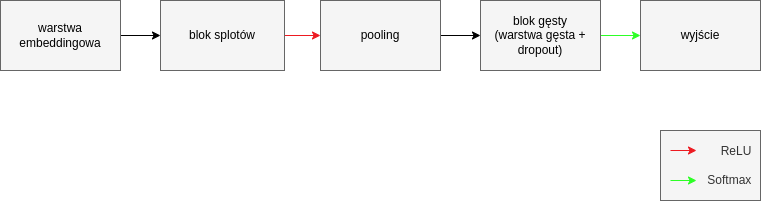
\includegraphics[width=0.8\linewidth]{img/architecture.png}
    \caption{Proponowana architektura klasyfikatora opartego warstwach splotowych.}
\end{figure}

Drugi model do celów porównawczych będzie oparty o wektor słów z pretrenowanego modelu
transformatorowego BERT\cite{bert}. Zmiana tyczy się tylko warstwy embeddingowej -- będą do niej
wprowadzone inne wektory.


\newpage
\section{Projekt implementacji}

\subsection{Pobieranie i przygotowywanie danych}

Przed przystąpieniem do trenowania modeli analizy wydźwięku należy zebrać odpowiednio liczny zbiór danych, które posłużą za dane testowe i treningowe dla implementowanego algorytmu.

\subsubsection{Skrypt do pozyskiwania danych z serwisu Amazon}

Ze względu na fakt, że istnieje wiele narzędzi pomagających w pobieraniu wpisów zintegrowanych z tym portalem, a także na łatwość przekładania liczby gwiazdek przyznanych produktowi przez użytkownika na wydźwięk pozytywny, negatywny bądź neutralny, zdecydowano się trenować model na danych pochodzących z serwisu Amazon.

Wybrano po kilka-kilkanaście produktów ze zadanych trzech kategorii i wyszukano je w serwisie Amazon. Następnie ich strony główne, zawierające recenzje stanowiące docelowy zestaw danych, pobrano w formie pliku HTML. W tym celu wykorzystano interfejs \textbf{ScraperAPI}, obsługujący serwery proxy, przeglądarki oraz CAPTCHA i tym samym pozwalający na uzyskanie HTML z dowolnej strony internetowej o znanym adresie URL za pomocą prostego wywołania w dowolnym języku. Zastosowanie takiego interfejsu lub innego, równoważnego narzędzia jest kluczowe w przypadku pobierania danych z serwisu, który implementuje zabezpieczenia przeciwko botom - inaczej żądania są blokowane.

Narzędzie, które zostało wykorzystane w celu wydobycia z otrzymanych w ten sposób dokumentów istotnych informacji to \textbf{Beautiful Soup} - biblioteka dostępna dla języka Python. Pozwala ona na przeszukiwanie plików HTML i XML przy pomocy prostych zapytań. Przykładowo, poniższy fragment kodu znajduje wszystkie elementy HTML będące znacznikiem span i dla których pole data-hook ma ustawioną wartość review-body: % ja nie wiem czy to jest do końca poprawne XD

\begin{lstlisting}
soup.find_all("span", {"data-hook": "review-body"})
\end{lstlisting}

Każdy z otrzymanych w poprzednim kroku plików przeszukano i dla każdego produktu wydobyto treści wszystkich widocznych na stronie recenzji razem z przydzielonymi gwiazdkami. Następnie przystąpiono do oznaczania sentymentów. Przyjęliśmy założenie, że ocena wynosząca 4 lub 5 gwiazdek oznacza wydźwięk pozytywny, ocena 3 - wydźwięk neutralny, a przyznanie 1 albo 2 gwiazdek wskazuje na wydźwięk negatywny. Tak oznaczone recenzje (treść - sentyment) zostały zgrupowane według kategorii produktu i zapisane w pliku w formacie csv.

\subsubsection{Opis pozyskanych danych}

Ostatecznie zebrano 251 recenzji:

\begin{center}
\begin{tabular}{ c c c }
 cell1 & cell2 & cell3 \\ 
 cell4 & cell5 & cell6 \\  
 cell7 & cell8 & cell9    
\end{tabular}
\end{center}

Rozkład klas jest równomierny w każdej kategorii.

\subsubsection{Preprocessing}

\subsection{Modele wykrywające wydźwięk}

%--------------------------------------------
% Literatura
%--------------------------------------------
\cleardoublepage % Zaczynamy od nieparzystej strony
\printbibliography



%--------------------------------------------
% Spisy (opcjonalne)
%--------------------------------------------
\pagestyle{plain}

\vspace{0.8cm}

\vspace{1cm}          % vertical space
%\listofappendicestoc  % Spis załączników

% Załączniki
%


\end{document}
